\tikzstyle{input_neuron}=[circle,draw=red!50,fill=orange!10,thick,minimum size=.2mm]
\tikzstyle{hidden_neuron}=[circle,draw=blue!50,fill=blue!10,thick,minimum size=1mm]
\tikzstyle{output_neuron}=[circle,draw=green!50,fill=green!20,thick,minimum size=1mm]
\tikzstyle{input}=[circle,draw=black!50,fill=black!20,thick,minimum size=.2mm]

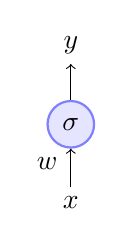
\begin{tikzpicture}

	\node (input0) at (10,5)  {$x$};
	\node [hidden_neuron] (neuron1) at (10,6)  {$\sigma$};
	\node (formula) at (9.7,5.5) {$w$};
	\node (output0)  at (10,7) {$y$};	
	\draw [->] (input0) -- (neuron1);
	\draw [->] (neuron1) -- (output0);
	
\end{tikzpicture}